\chapter{KAN у контексті комп'ютерного зору}

\section{Класичні конволюційні нейронні мережі}

Нагадаємо, що під час нашої попередньої дискусії, ми розглядали лише
мультишарові перцептрони (MLP), що описуються рекурентним співвідношенням
$\mathbf{x}^{\langle \ell+1 \rangle} = \phi(\boldsymbol{W}^{\langle \ell
\rangle}\mathbf{x}^{\langle \ell \rangle} + \boldsymbol{\beta}^{\langle \ell
\rangle})$. Проте, як видно, в цьому рівнянні кожне проміжне значення, включно з
початковим --- це вектор. Уявімо, що нам потрібно побудувати нейронну мережу на
основі зображення, яке є двовимірним масивом пікселів. Природньо розв'язати цю
задачу наступним чином: просто розгорнемо зображення в одновимірний вектор, а
потім застосуємо до нього MLP. І саме таким чином були побудовані одні з перших
моделей машинного навчання на зображеннях. Зокрема, навіть до розвитку глибокого
навчання, такий спосіб був використаний у біометричних системах для
розпізнавання облич Eigenface \cite{eigenface} та Fisherface \cite{fisherface},
де зображення обличчя перетворювалося в одновимірний вектор, а потім
застосовувався алгоритм PCA або LDA для зменшення розмірності \cite{pca}.

Проте, як показує сучасна практика, такий підхід не є оптимальним. Найбільша 
проблема наступна: нехай задача є бінарною класифікацією над зобарежннями 
розміру $100 \times 100$. У якості нейронної мережі, ми під'єднаємо 
вхідний шар до прихованого шару зі $100$ нейронами, що в свою чергу 
під'єднаний до виходу. Тоді, кількість параметрів у моделі буде 
$100 \times 100 \times 100 = 1 \, \text{млн}$, хоча модель містить 
буквально один малий прихований шар. 

Річ у тому, що зв'язків між нейронами у вхідному та прихованому шарах
дуже багато і, як показує практика, більшість з них є зайвими. Нам 
потрібно побудувати таку функцію переходу, яка б враховувала 
просторову структуру зображення. Для цього, ми можемо
використати концепцію \textit{згортки} (convolution).

Історично, згортки виникли як наступний оператор над простором 
функцій: нехай маємо функції $f(x)$ та $g(x)$, тоді згорткою 
називають вираз
\begin{equation}
    (f \star g)(x) = \int_{-\infty}^{\infty} f(\tau) g(x - \tau) d\tau.
\end{equation}

Проте, що в комп'ютерному зорі, ми будемо використовувати дискретну версію
згортки, причому в основному для трьохвимірних масивів. Почнемо, проте, з 
двовимірної версії. Визначимо згортку двохвимірного зображення наступним чином.
\begin{definition}
    Маючи зображення $\boldsymbol{X} \in \mathbb{R}^{W \times H}$ та так званий
    \textit{фільтр} або \textit{ядро} $\boldsymbol{K} \in \mathbb{R}^{f \times
    f}$, результатом будемо називати нове зображення
    $\boldsymbol{Y}=\boldsymbol{K} \star \boldsymbol{X}$ розміру $(W-f+1) \times
    (H-f+1)$, яке визначається як
    \begin{equation}
        Y_{i,j} = \sum_{u=0}^{f-1} \sum_{v=0}^{f-1} X_{i+u,j+v} \cdot K_{u,v}.
    \end{equation}
\end{definition}

Геометрично, фільтр накладається на зображення, починаючи з верхнього лівого
кута, і переміщається по зображенню, обчислюючи нове значення пікселя шляхом
обчислення скалярного добутку між фільтром та частиною зображення, на яку
він накладається. Таким чином, нове зображення є результатом застосування
фільтра до всіх можливих позицій у зображенні. Приклад застосування фільтра показано 
на Рисунку \ref{fig:conv_example}.

\begin{figure}
\[
\left[\begin{array}{ccccccc}
  0 & 1 & 1 & \mymark{TL1}{1}\mysmall{1} & 0\mysmall{0} & \mymark{TR1}{0}\mysmall{1} & 0\\
  0 & 0 & 1 &               1\mysmall{0} & 1\mysmall{1} &               0\mysmall{0} & 0\\
  0 & 0 & 0 & \mymark{BL1}{1}\mysmall{1} & 1\mysmall{0} & \mymark{BR1}{1}\mysmall{1} & 0\\
  0 & 0 & 0 & 1 & 1 & 0 & 0\\
  0 & 0 & 1 & 1 & 0 & 0 & 0\\
  0 & 1 & 1 & 0 & 0 & 0 & 0\\
  1 & 1 & 0 & 0 & 0 & 0 & 0\\
\end{array}\right]
\star
\left[\begin{array}{ccc}
  \mymark{TL2}{1} & 0 & \mymark{TR2}{1}\\
  0  & 1 &              0 \\
  \mymark{BL2}{1} & 0 & \mymark{BR2}{1}
\end{array}\right]
=
\left[\begin{array}{ccccccc}
  1 & 4 & 3 & \mymark{C}{4} & 1\\
  1 & 2 & 4 & 3 & 3\\
  1 & 2 & 3 & 4 & 1\\
  1 & 3 & 3 & 1 & 1\\
  3 & 3 & 1 & 1 & 0
\end{array}\right]
\]
\begin{tikzpicture}[overlay, remember picture,
    myedge1/.style={dashed, opacity=.3, blue},
    myedge2/.style={dashed, opacity=.3, green!40!black}]

  %% Draw boxes
  \draw[red, fill=red, fill opacity=.1, very thick]   (TL1.north west) rectangle (BR1.south east);
  \draw[blue, fill=blue, fill opacity=.1, very thick] (TL2.north west) rectangle (BR2.south east);
  \draw[green!60!black, fill=green, fill opacity=.1, very thick] (C.north west) rectangle (C.south east);

  %% Draw blue lines
  \draw[myedge1] (TL1.north west) -- (TL2.north west);
  \draw[myedge1] (BL1.south west) -- (BL2.south west);
  \draw[myedge1] (TR1.north east) -- (TR2.north east);
  \draw[myedge1] (BR1.south east) -- (BR2.south east);

  %% Draw green lines
  \draw[myedge2] (TL2.north west) -- (C.north west);
  \draw[myedge2] (BL2.south west) -- (C.south west);
  \draw[myedge2] (TR2.north east) -- (C.north east);
  \draw[myedge2] (BR2.south east) -- (C.south east);
\end{tikzpicture}
\caption{Приклад згортки зображення $7 \times 7$ з фільтром $3 \times 3$.}
\label{fig:conv_example}
\end{figure}

Коли ми тренуємо нейронну мережу, то сподіваємося, що вона навчиться 
правильно підбирати коефіцієнти у фільтрах. Наприклад, нейронна мережа 
може навчитися виділяти краї, текстури або інші важливі ознаки зображення.
Приклад показано на Рисунку \ref{fig:sobel}: якщо використати 
так звані фільтри Собеля:
\begin{equation}
    \boldsymbol{G}_X = \begin{bmatrix}
        -1 & 0 & +1 \\
        -2 & 0 & +2 \\
        +1 & +2 & +1 
    \end{bmatrix}, \quad \boldsymbol{G}_Y = \begin{bmatrix}
        -1 & -2 & -1 \\
        0 & 0 & 0 \\
        +1 & +2 & +1
    \end{bmatrix},
\end{equation}

що виділяють вертикальні та горизонтальні краї відповідно, а далі обрахувати
зображення $\boldsymbol{Y} := \sqrt{(\boldsymbol{G}_X \star \boldsymbol{X})^2 +
(\boldsymbol{G}_Y \star \boldsymbol{X})^2}$ (де зазначені операції робляться
по-елементно), то отримаємо виділені контури на зображенні.

\begin{figure}
    \centering
    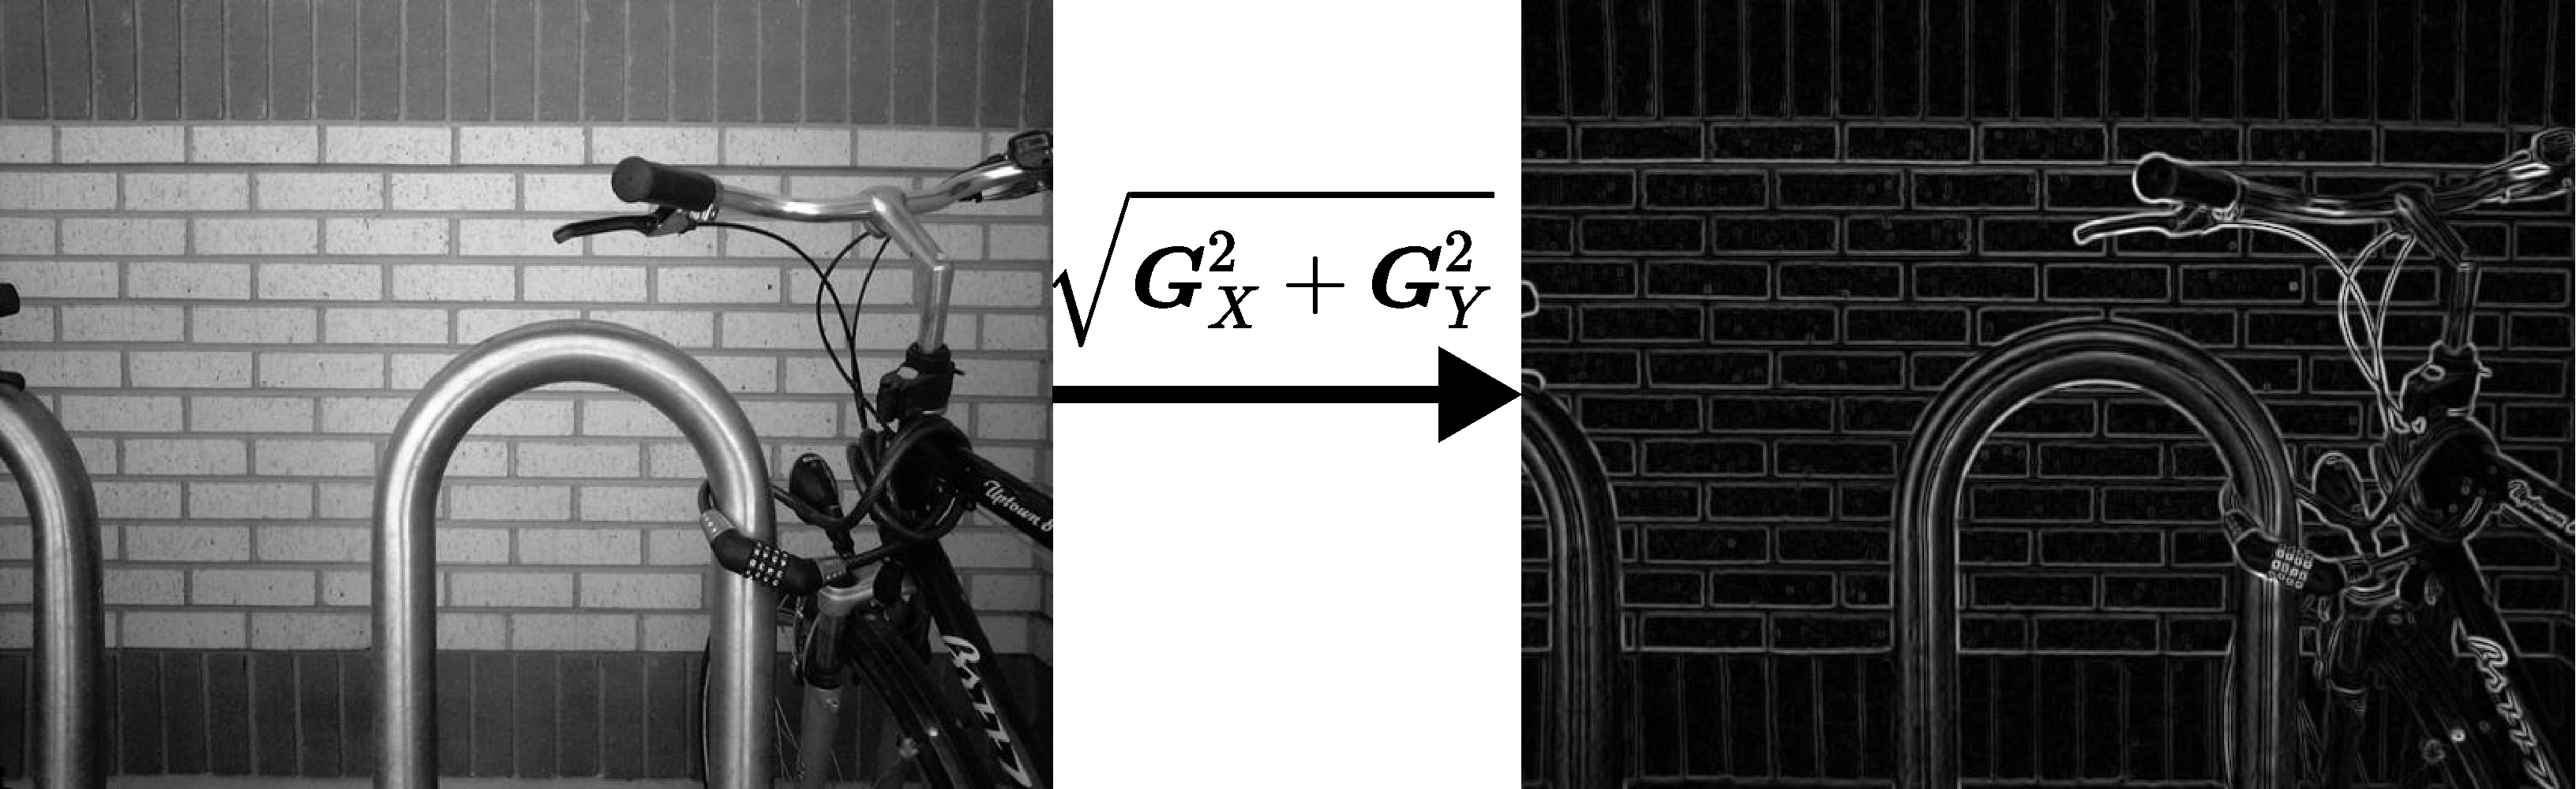
\includegraphics[width=1.0\linewidth]{figures/convolutions/sobel.pdf}
    \caption{Приклад виділення країв на зображенні за допомогою накладання
    конволюцій (фільтри Собеля). Ліворуч --- оригінальне зображення, праворуч
    --- виділені краї.}
    \label{fig:sobel}
\end{figure}

\section{Згортки у нейронних мережах}

Проте, зазначена вище процедура була визначена лише для двовимірних
зображень та наявності одного фільтра. У нейронних мережах ми
зазвичай маємо справу з тривимірними масивами: наприклад, кольорове 
зображення є тривимірним масивом розміру $W \times H \times 3$, де
$3$ --- це кількість кольорових каналів (червоний, зелений, синій).
Тому, ми повинні розширити визначення згортки на тривимірні масиви.

\begin{definition}
    Нехай $\boldsymbol{X} \in \mathbb{R}^{W \times H \times C}$ --- набір з $C$
    зображень (кількість каналів) розміру $W \times H$, та $\boldsymbol{K} \in
    \mathbb{R}^{f \times f \times C \times C'}$ --- набір з $C'$ фільтрів (ядер)
    розміру $f \times f \times C$. Тоді, результатом згортки буде нове
    зображення (тензор) $\boldsymbol{Y} \in \mathbb{R}^{(W-f+1) \times (H-f+1)
    \times C'}$, яке визначається як
    \begin{equation}
        Y_{i,j,k} = \sum_{u=0}^{f-1} \sum_{v=0}^{f-1} \sum_{c=0}^{C-1} X_{i+u,j+v,c} \cdot K_{u,v,c,k}.
    \end{equation}
\end{definition}

Тут інтуїція дуже схожа: беремо фільтр $f \times f \times C$, накладаємо на
частину зображення $W \times H \times C$, обчислюємо скалярний добуток та
отримуємо нове значення одного пікселя. Проходимось по всьому об'єму, щоб
отримати зображення розміру $(W-f+1) \times (H-f+1)$. Далі ми це повторюємо для
всіх фільтрів $C'$, щоб отримати вже тензор $\mathbb{R}^{(W-f+1) \times (H-f+1)
\times C'}$. 


Проте, як можна помітити, задані операції конволюції ніяк не розв'язують нашу
початкову проблему: розмір входу та виходу майже ніяк не змінюються (оскільки на
практиці розмір фільтру $f \ll W,H$). Тому, нам потрібні інструменти, які
дозволять зменшувати розмір зображення. Для цього введемо декілька інструментів.
\begin{itemize}
    \item \textbf{Паддінг} (padding) --- це додавання нулів до країв зображення.
    Це дозволяє зберегти розмір зображення незмінним під час згортки (себто, 
    якщо у нас є зображення $W \times H$ та фільтр $f \times f$, то після
    паддінгу зображення до $(W+f-1) \times (H+f-1)$, ми отримаємо нове
    зображення початкового розміру $W \times H$). Ця операція не зменшує 
    розмір зображення, але працювати з нею стає зручніше надалі.
    \item \textbf{Страйд} (stride) --- це крок, на який фільтр переміщується по
    зображенню. Зазвичай, ми використовуємо $s=1$ або $s=2$ або в рідкісних
    випадках $s=3$. З використанням паддінгу та страйду $s$, ми можемо зменшити
    розмір зображення в кожному каналі з $W \times H$ до $\frac{W}{s} \times
    \frac{H}{s}$.
    \item \textbf{Пулінг} (pooling) --- це операція, яка зменшує розмір
    зображення шляхом обчислення статистики (максимуму або середнього) над
    невеликими ділянками зображення. Наприклад, якщо ми маємо $2 \times 2$
    ділянку зображення, то ми можемо взяти максимум або середнє значення
    пікселів у цій ділянці і замінити всю ділянку на це значення.
\end{itemize}

Таким чином, ідея побудови конволюційної нейронної мережі полягає в тому, що ми
будемо використовувати згортки для виділення ознак з зображення, а потім
зменшувати розмір зображення за допомогою пулінгу або страйду. Приклад
конволюційної нейронної мережі показано на Рисунку \ref{fig:convnet}. Як видно,
ми маємо декілька шарів конволюційних фільтрів, які виділяють ознаки з
зображення, а потім зменшують розмір зображення за допомогою пулінгу. Після
цього, ми використовуємо повнозв'язний шар, щоб отримати остаточну класифікацію
зображення. 

\begin{figure}
    \centering
    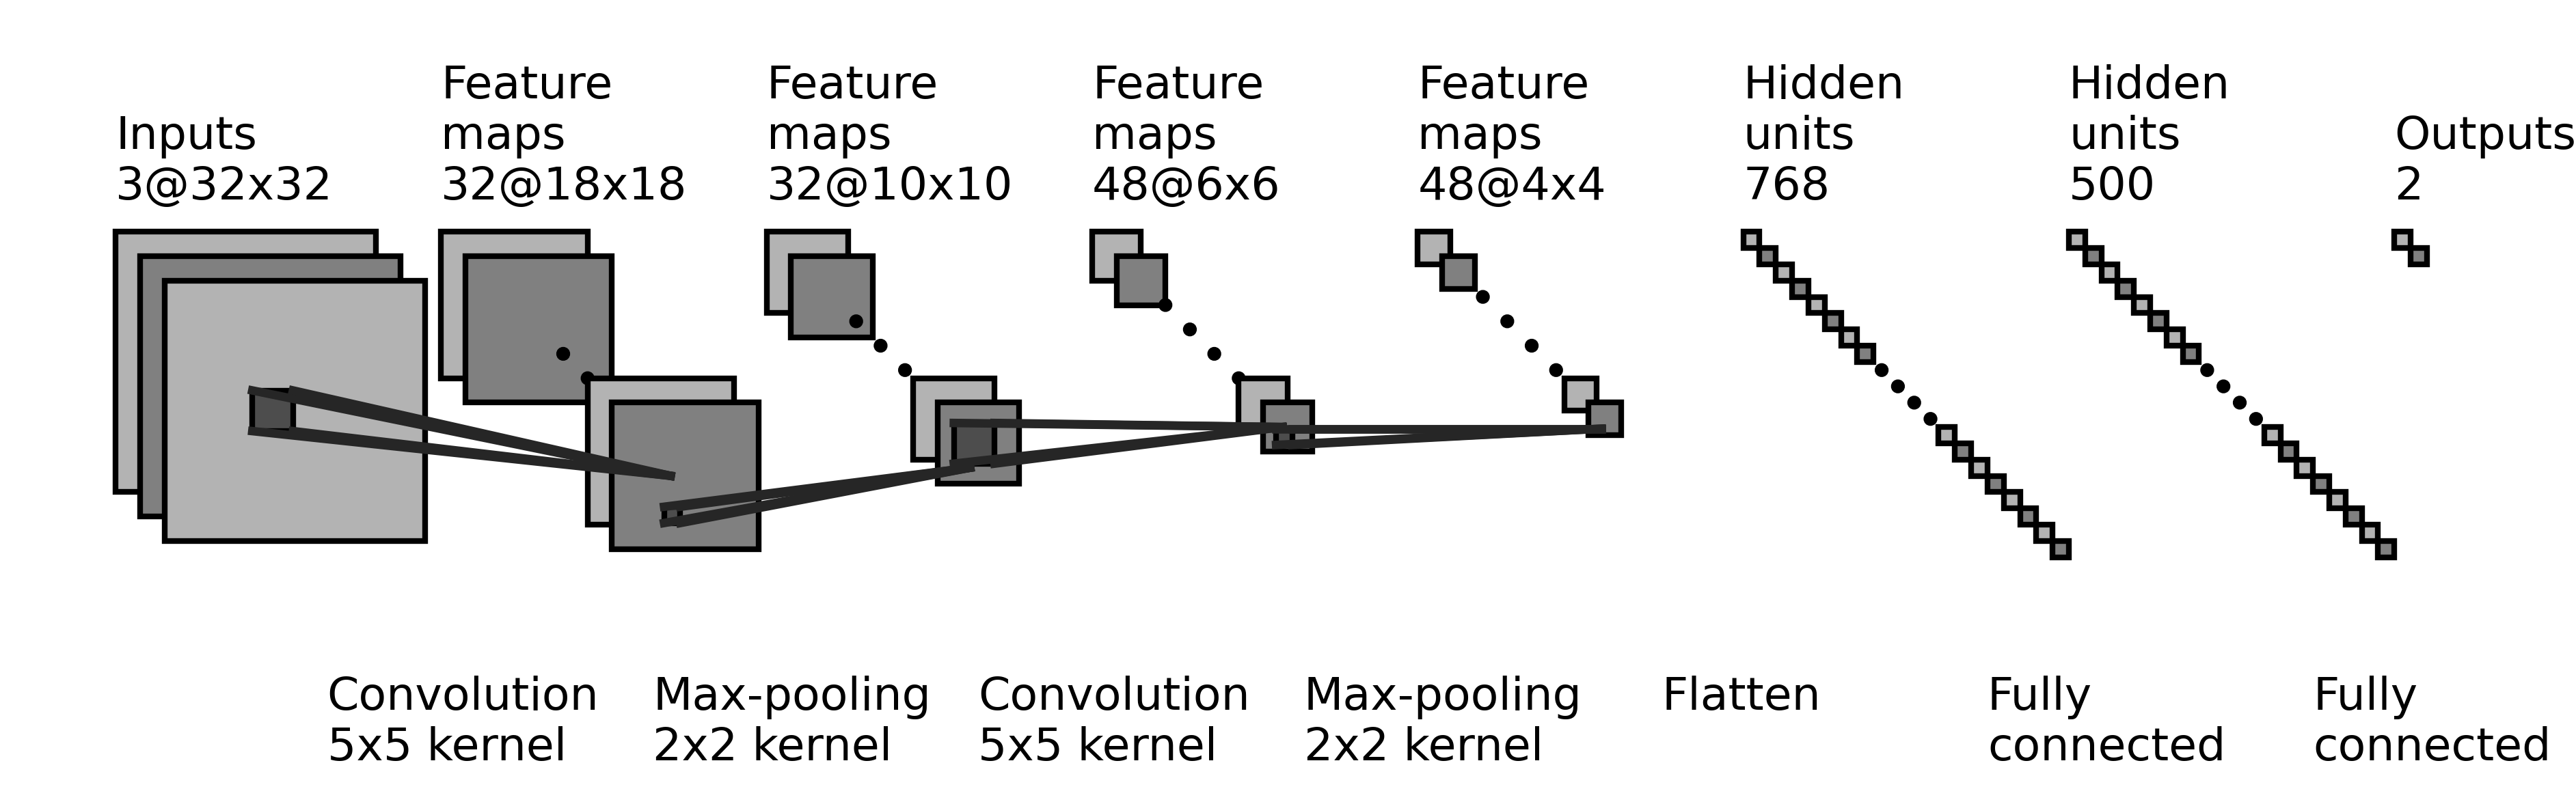
\includegraphics[width=1.0\linewidth]{figures/convolutions/convnet_fig.png}
    \caption{Приклад глибокої конволюційної нейронної мережі}
    \label{fig:convnet}
\end{figure}

Єдине ключове питання, що ми оминули --- це як саме накладати нелінійність 
у конволюційних нейронних мережах. Дійсно, якщо просто взяти композицію 
згорткових шарів, то ми отримаємо одне лише лінійне перетворення.
Тому, ми повинні накладати нелінійність після кожної згортки. Це можна 
зробити дуже просто: при кожному обрахунку суми $\sum_{u,v,c}X_{i+u,j+v,c}K_{u,v,c,k}$,
ми будемо накладати нелінійність $\phi$ на результат та додавати 
зсув $\beta_{i,j,k}$.
\begin{definition}
    Нехай $\boldsymbol{X} \in \mathbb{R}^{W \times H \times C}$ --- набір з $C$
    зображень (кількість каналів) розміру $W \times H$, та $\boldsymbol{K} \in
    \mathbb{R}^{f \times f \times C \times C'}$ --- набір з $C'$ фільтрів (ядер)
    розміру $f \times f \times C$. Тоді, результатом згортки з нелінійністю
    $\phi$ та страйдом $s$ буде нове зображення $\boldsymbol{Y} \in
    \mathbb{R}^{\frac{W}{s} \times \frac{H}{s} \times C'}$, яке визначається як
    \begin{equation}
        \textcolor{blue}{Y_{i,j,k} = \phi\left(\sum_{u=0}^{f-1} \sum_{v=0}^{f-1} \sum_{c=0}^{C-1} X_{i+u,j+v,c} K_{u,v,c,k} + \beta_{i,j,k}\right).}
    \end{equation}
\end{definition}

Ця формула є ключовою для побудови конволюційних нейронних мереж і ми 
будемо орієнтуватись на неї у подальшій дискусії. 

\section{Згортки Колмогорова-Арнольда}\label{section:kolmogorov}

Нарешті, ми дійшли до найцікавішого: побудова конволюцій Колмогорова-Арнольда.
Наша конструкція вмотивована конструкцією \cite{kan-cnn}, котру ми в цій роботі
проаналізуємо та дослідимо детальніше. Отже, як і в оригінальній повнозв'язаній 
нейронні мережі, ідея полягає в тому, що ми будемо використовувати 
параметризовані функції замість скалярних значень. Таким чином, 
кожен елемент в фільтрі буде окремою функцією, що ми будемо накладати.
Різницю між звичайною згорткою та згорткою Колмогорова-Арнольда можна
побачити на Рисунку \ref{fig:kan_conv}.
\begin{figure}
\noindent
    \begin{minipage}{0.48\linewidth}
    \textcolor{blue}{
    \begin{equation*}
    \boldsymbol{K}_{\text{MLP}} = \begin{bmatrix}
        k_{1,1} & \cdots & k_{1,f} \\
        \vdots & \ddots & \vdots \\
        k_{f,1} & \cdots & k_{f,f}
    \end{bmatrix} \in \mathbb{R}^{f \times f}
    \end{equation*}
    MLP згортка $f \times f$, складається з $f^2$ параметрів $k_{i,j} \in \mathbb{R}$.}
    \end{minipage}
    \hfill
    \begin{minipage}{0.48\linewidth}
    \textcolor{purple}{
    \begin{equation*}
    \boldsymbol{K}_{\text{KAN}} = \begin{bmatrix}
        \phi_{1,1}(x) & \cdots & \phi_{1,f}(x) \\
        \vdots & \ddots & \vdots \\
        \phi_{f,1}(x) & \cdots & \phi_{f,f}(x)
    \end{bmatrix} \in \mathcal{F}^{f \times f}
    \end{equation*}
    KAN згортка $f \times f$, складається з $f^2$ функцій
    $\phi_{\boldsymbol{i}}(x)=\omega_{\boldsymbol{i},\beta}\beta(x)+\omega_{\boldsymbol{i},S} S(x)$.}
    \end{minipage}
    \caption{Порівняння між звичайною згорткою та згорткою Колмогорова-Арнольда.}
    \label{fig:kan_conv}
\end{figure}

Таким чином, дамо наступне визначення згортки Колмогорова-Арнольда.
\begin{definition}
    Нехай $\boldsymbol{X} \in \mathbb{R}^{W \times H \times C}$ --- набір з $C$
    зображень (кількість каналів) розміру $W \times H$, та $\boldsymbol{K} \in
    \mathcal{F}^{f \times f \times C \times C'}$ --- набір з $C'$ фільтрів
    (ядер) розміру $f \times f \times C$, що складаються з параметризованих
    сплайнів. Тоді, результатом згортки буде нове зображення $\boldsymbol{Y} \in
    \mathbb{R}^{W \times H \times C}$:
    \begin{equation}
        \textcolor{purple}{Y_{i,j,k} = \sum_{u=0}^{f-1} \sum_{v=0}^{f-1} \sum_{c=0}^{C'-1} \phi_{u,v,c,k}(X_{i+u,j+v,k})},
    \end{equation}
    причому кожен $\phi_{\boldsymbol{i}}(x) = \omega_{\boldsymbol{i},\beta}\beta(x)+\beta_{\boldsymbol{i},S} \sum_j c_{\boldsymbol{i},j}B_j(x)$,
    $\beta(x)=x\sigma(x)$.
\end{definition}

Реалізацію згортки Колмогорова-Арнольда можна знайти в Додатку \ref{appendix:c-ckan-code}.

\subsection{Мотивація конволюцій Колмогорова-Арнольда}

В MLP згортках ми вже бачили геометричний сенс: наприклад, фільтр при правильній
побудові може виділяти краї або локальну геометрію зображення, проте складніші
висновки можуть бути отримані лише після кількох конволюцій поспіль.

Головна користь KAN згорток, що ми вбачаємо, наступна: KAN згортки дозволяють
будувати такі фільтри, що мають значно складнішу поведінку, ніж MLP згортки.
Наприклад, у роботі \cite{kan-cnn} наводять наступний приклад: нехай ми задали
поріг $\tau$ і усі пікселі, що мають більшу яскравість ніж $\tau$, стають ще
світлішими, а усі інші стають темнішими. Таким чином, наша функція $\phi_{i,j}$
виглядає як:
\begin{equation*}
    \phi_{i,j}(x) = \begin{cases}
        \alpha_{\text{bright}}\cdot x, & \text{якщо } x \geq \tau_{i,j}, \\
        \alpha_{\text{dark}}\cdot x, & \text{інакше.}
    \end{cases}
\end{equation*}

Помітимо, що таке перетворення зображення ми б не змогли реалізувати за
допомогою звичайної MLP згортки.

\section{$B$-сплайни}

Як ми вже зазначали, в якості активаційної функції автори \cite{kan} 
використовують $B$-сплайни, тому варто розглянути їх дещо детальніше.

$B$-сплайни --- це функції, які використовуються для апроксимації
функцій та побудови кривих. Вони є частиною більш загальної категорії
\textit{сплайнів}, які є функціями, що складаються з декількох поліномів,
які з'єднані разом у певних точках, що називаються \textit{вузлами} (knots).
$B$-сплайни є особливим випадком сплайнів, які мають певні властивості,
такі як неперервність та гладкість, що робить їх дуже корисними для
апроксимації функцій та побудови кривих.

В нашому конкретному випадку, ми будемо використовувати $B$-сплайни порядку $d$
для апроксимації функій у вигляді суми $S(x) = \sum_{i}c_iB_{i,d}(x)$ (з межами
суми ми визначимось дещо пізніше), де функції $B_{i,d}(x)$ природньо називають
\textit{базисними функціями} $B$-сплайнів порядку $d$. Вони визначаються
рекурсивно за допомогою формули Кокс-де Бьорна (Cox-de Boor recursion formula)
\cite{b-splines} над вузлами $x_0, x_1, \ldots, x_n$:
\begin{gather}
    B_{i,0}(x) = \begin{cases}
        1, & \text{якщо } x_i \leq x < x_{i+1}, \\
        0, & \text{інакше.}
    \end{cases} \\
    B_{i,d}(x) = \frac{x-x_i}{x_{i+d}-x_i}B_{i,d-1}(x) + \frac{x_{i+d+1}-x}{x_{i+d+1}-x_{i+1}}B_{i+1,d-1}(x), \quad d > 0
\end{gather}

Проілюструємо ці базисні функції на прикладі $B$-сплайнів порядку $0 \leq d \leq
3$ на множині вузлів $\{0,\dots,6\}$: дивись Рисунок \ref{fig:b-splines}.
\begin{figure}
    \begin{tabular}{cc}
      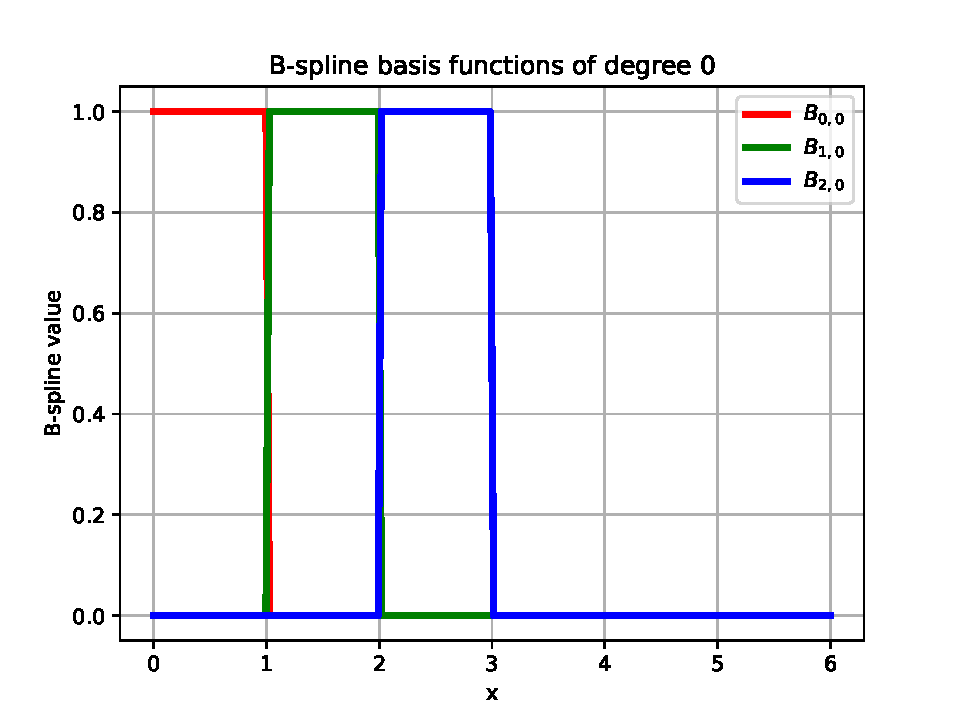
\includegraphics[width=0.5\textwidth]{code/splines/bspline_degree_0.pdf} &   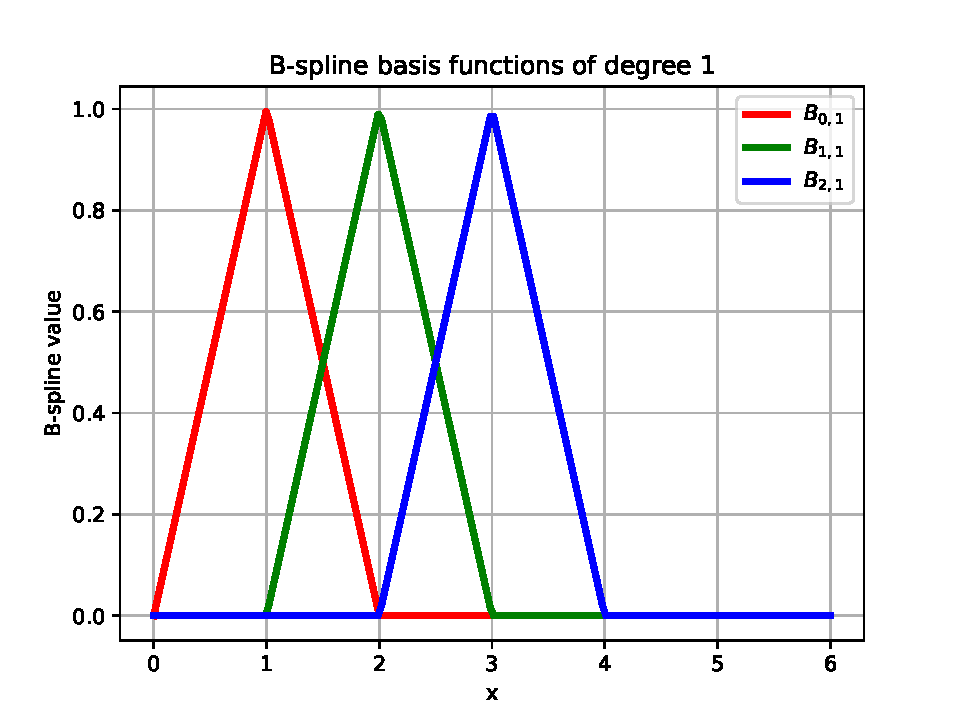
\includegraphics[width=0.5\textwidth]{code/splines/bspline_degree_1.pdf} \\
      Степінь $d=0$ & Степінь $d=1$ \\
      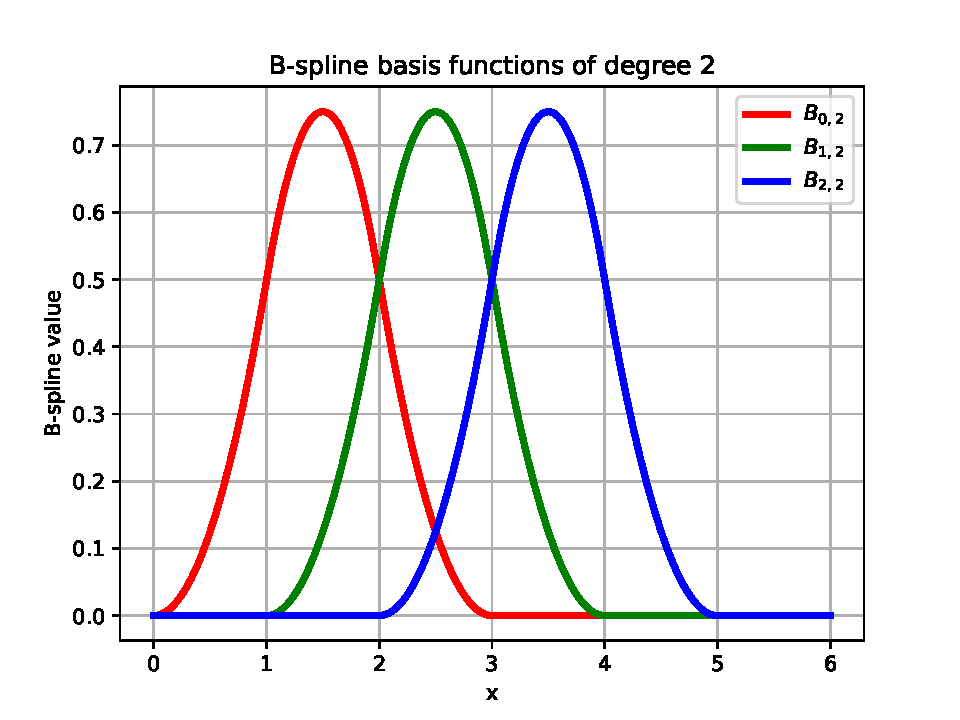
\includegraphics[width=0.5\textwidth]{code/splines/bspline_degree_2.pdf} &   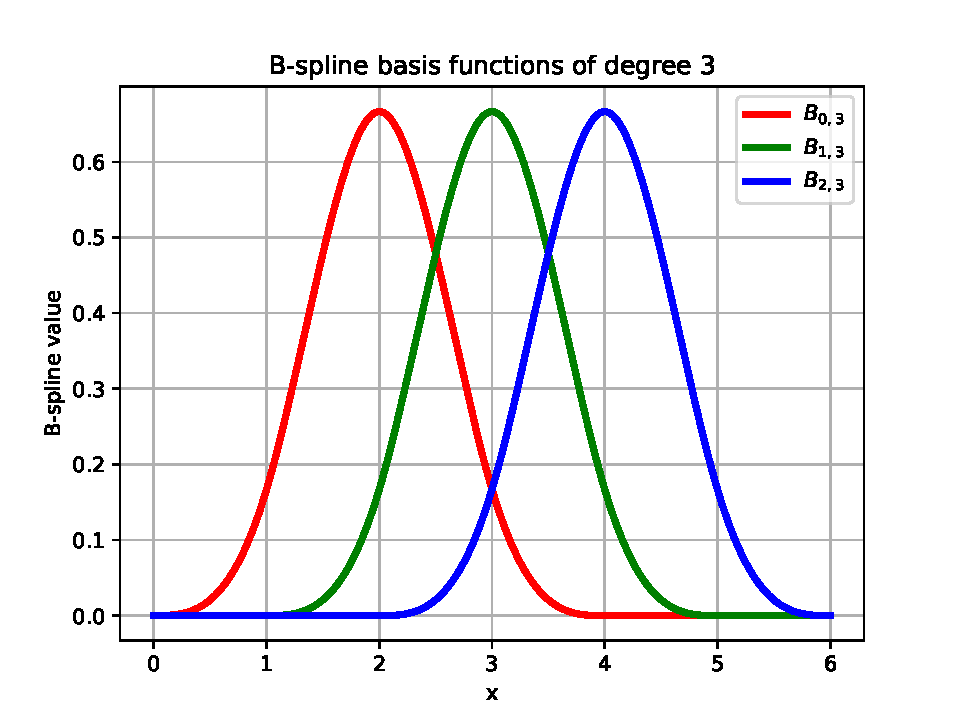
\includegraphics[width=0.5\textwidth]{code/splines/bspline_degree_3.pdf} \\
      Степінь $d=2$ & Степінь $d=3$
    \end{tabular}
    \caption{Три базисних $B$-сплайн полінома $\{B_{i,d}(x)\}_{i \in \{0,1,2\}}$
    для степенів поліномів $d \in \{0,1,2,3\}$ на множині вузлів $\{0,\dots,6\}$.}
    \label{fig:b-splines}
\end{figure}

Бачимо, що базисні функції $B_{i,d}(x)$ є неперервними та гладкими функціями,
які мають значення $0$ в усіх точках, окрім відрізку $(x_i,x_{i+d+1})$. Більш
того, можна показати, що $B_{i,d}(x) \in \mathcal{C}^{d-1}(\mathbb{R})$. Як бачимо, чим
більший порядок $d$, тим більший відрізок ``покриває'' базисний поліном
$B_{i,d}(x)$. Саме тому при $n$ вузлах, нам доступні лише 
$n-d-1$ базисних функцій $B_{i,d}(x)$. 

В оригінальній статті пропонується обирати $d=3$ та побудувати сітку над
областтю $[-1,1]$, розбивши її на $n$ рівних частин. Таким чином, маємо вузли
$x_i = -1 + 2i/n$ для $i=0,\dots,n$. Щоб отримати $n+d$ базисних функцій, стаття
пропонує розширити сітку в обидва боки, додавши по $d$ вузлів з обох сторін.
Таким чином, отримуємо наступний вигляд апроксимації:
\begin{equation}
    \widehat{f}(x|\boldsymbol{c}) = \sum_{i=1}^{n+d} c_i B_{i,d}(x), \quad x \in [-1,1].
\end{equation}

Продемонструємо, як відбувається пошук коефіцієнтів $\{c_i\}_{0 < i \leq n+d}$
на практиці. Нехай нам задана певна функція $f(x)$ і ми хочемо її апроксимувати
за допомогою $B$-сплайнів. Таку задачу можна розв'язати за допомогою методу
найменших квадратів
\begin{align}
    \widehat{\boldsymbol{c}} &= \argmin_{\boldsymbol{c} \in \mathbb{R}^{n+d}} \sum_{i=1}^{n+d} \left(f(x_i) - \widehat{f}(x_i|\boldsymbol{c})\right)^2 \\
    &= \argmin_{\boldsymbol{c} \in \mathbb{R}^{n+d}} \sum_{i=1}^{n+d} \left(f(x_i) - \sum_{j=1}^{n+d} c_j B_{j,d}(x_i)\right)^2
\end{align}

Як і у випадку з лінійною регресією, це зводиться до розв'язання системи
лінійних рівнянь. В якості більш цікавого прикладу, візьмемо функцію $f(x) = x^2
e^{x/8} \sin(2\pi x)$. Далі, згенеруємо $100$ точок на відрізку $[-1,1]$, де $y$
координата кожної точки $x_i$ буде задана як $f(x_i)+\varepsilon$, де
$\varepsilon \sim \mathcal{N}(0,0.1)$ --- випадковий шум з відносно малою
дисперсією. На Рисунку \ref{fig:bspline_approx} показано результат апроксимації
за допомогою $B$-сплайнів порядку $d=3$ з $n=15$ вузлами, де ми шукали 
коефіцієнти за допомогою градієнтного спуску (метод Adam \cite{adam}) 
з метрикою середньоквадратичної помилки (MSE). Як видно, отримана
апроксимація дуже близька до оригінальної функції, що свідчить про
досить хорошу якість апроксимації.

Реалізацію модуля $B$-сплайнів можна знайти в додатку \ref{appendix:b-spline-code}.

\begin{figure}
    \centering
    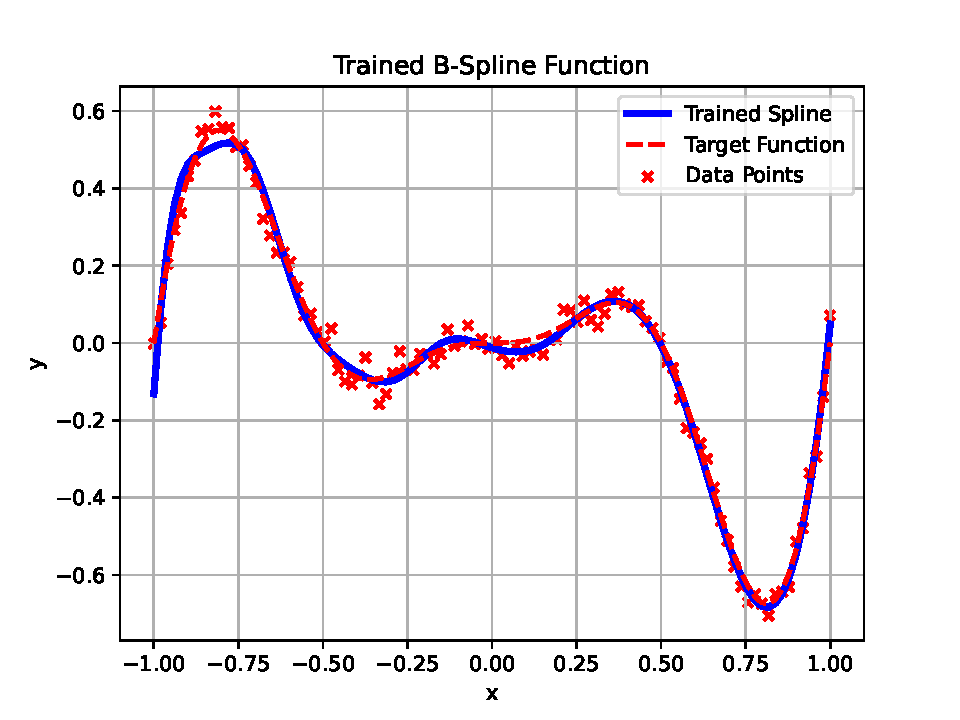
\includegraphics[width=0.8\linewidth]{figures/trained_spline.pdf}
    \caption{Приклад апроксимації функції $f(x) = x^2e^{x/8} \sin 2\pi x$ за
    допомогою $B$-сплайнів порядку $d=3$ з $n=10$ вузлами.}
    \label{fig:bspline_approx}
\end{figure}

